\documentclass{beamer}\usepackage[]{graphicx}\usepackage[]{color}
%% maxwidth is the original width if it is less than linewidth
%% otherwise use linewidth (to make sure the graphics do not exceed the margin)
\makeatletter
\def\maxwidth{ %
  \ifdim\Gin@nat@width>\linewidth
    \linewidth
  \else
    \Gin@nat@width
  \fi
}
\makeatother

\definecolor{fgcolor}{rgb}{1, 0.894, 0.769}
\newcommand{\hlnum}[1]{\textcolor[rgb]{0.824,0.412,0.118}{#1}}%
\newcommand{\hlstr}[1]{\textcolor[rgb]{1,0.894,0.71}{#1}}%
\newcommand{\hlcom}[1]{\textcolor[rgb]{0.824,0.706,0.549}{#1}}%
\newcommand{\hlopt}[1]{\textcolor[rgb]{1,0.894,0.769}{#1}}%
\newcommand{\hlstd}[1]{\textcolor[rgb]{1,0.894,0.769}{#1}}%
\newcommand{\hlkwa}[1]{\textcolor[rgb]{0.941,0.902,0.549}{#1}}%
\newcommand{\hlkwb}[1]{\textcolor[rgb]{0.804,0.776,0.451}{#1}}%
\newcommand{\hlkwc}[1]{\textcolor[rgb]{0.78,0.941,0.545}{#1}}%
\newcommand{\hlkwd}[1]{\textcolor[rgb]{1,0.78,0.769}{#1}}%
\let\hlipl\hlkwb

\usepackage{framed}
\makeatletter
\newenvironment{kframe}{%
 \def\at@end@of@kframe{}%
 \ifinner\ifhmode%
  \def\at@end@of@kframe{\end{minipage}}%
  \begin{minipage}{\columnwidth}%
 \fi\fi%
 \def\FrameCommand##1{\hskip\@totalleftmargin \hskip-\fboxsep
 \colorbox{shadecolor}{##1}\hskip-\fboxsep
     % There is no \\@totalrightmargin, so:
     \hskip-\linewidth \hskip-\@totalleftmargin \hskip\columnwidth}%
 \MakeFramed {\advance\hsize-\width
   \@totalleftmargin\z@ \linewidth\hsize
   \@setminipage}}%
 {\par\unskip\endMakeFramed%
 \at@end@of@kframe}
\makeatother

\definecolor{shadecolor}{rgb}{.97, .97, .97}
\definecolor{messagecolor}{rgb}{0, 0, 0}
\definecolor{warningcolor}{rgb}{1, 0, 1}
\definecolor{errorcolor}{rgb}{1, 0, 0}
\newenvironment{knitrout}{}{} % an empty environment to be redefined in TeX

\usepackage{alltt}
\usepackage{../371g-slides}
\title{Model Building}
\subtitle{Lecture 14}
\author{STA 371G}
\IfFileExists{upquote.sty}{\usepackage{upquote}}{}
\begin{document}
  
  

  \frame{\maketitle}

  % Show outline at beginning of each section
  \AtBeginSection[]{ 
    \begin{frame}<beamer>
      \tableofcontents[currentsection]
    \end{frame}
  }

  %%%%%%% Slides start here %%%%%%%

  \begin{darkframes}
    
    
    \begin{frame}{There is a Primary Care Physician Shortage in Texas!}
      \begin{center}
        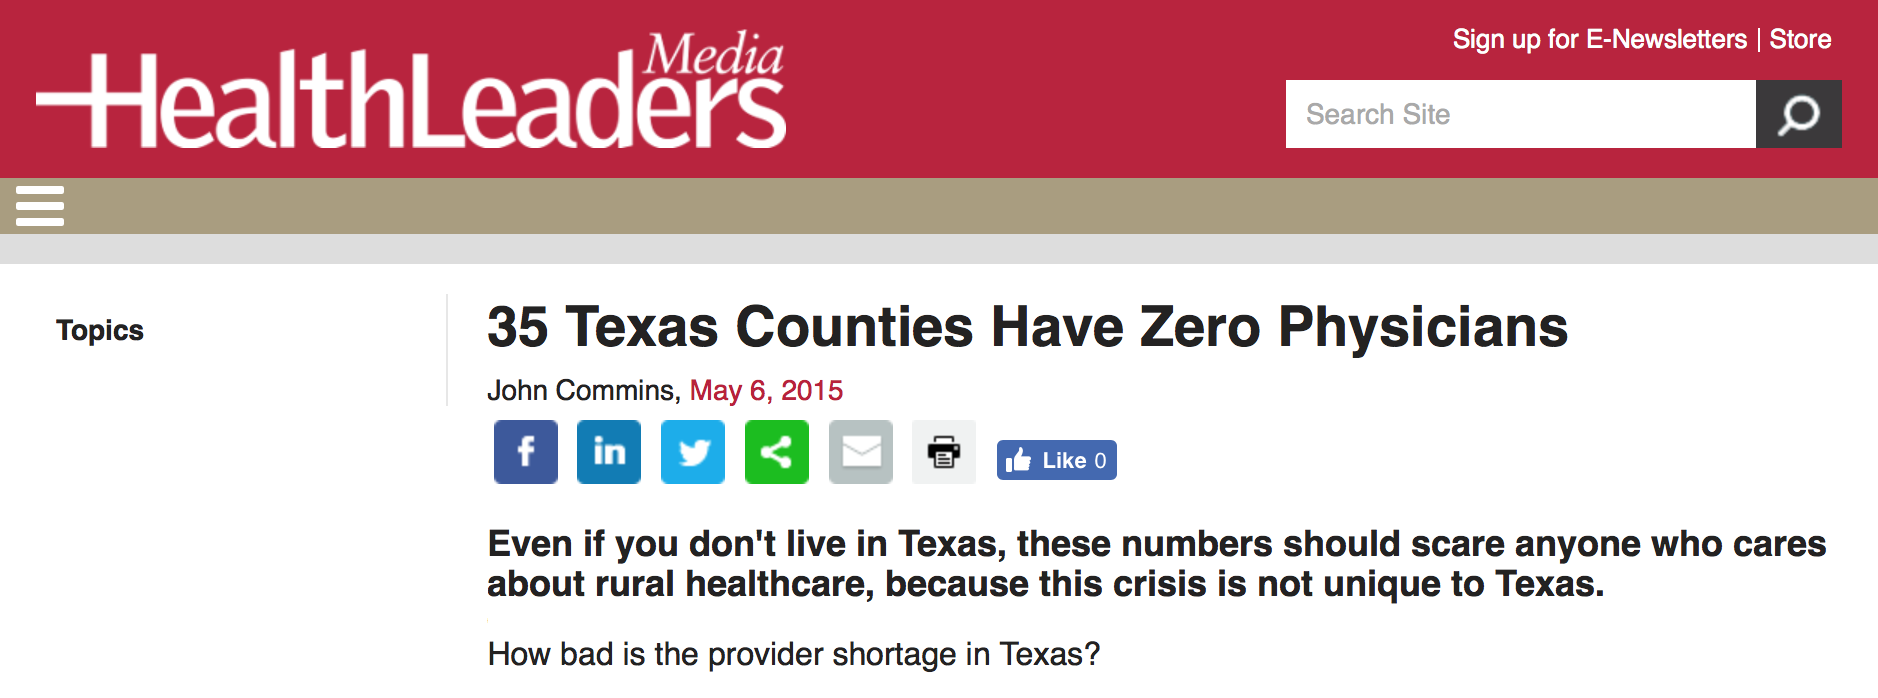
\includegraphics[width=3.8in]{DocShortage} \\
      \end{center} \pause

      \begin{center}
        {What might explain this? There are many potential predictors!}
      \end{center} 

      \begin{columns}[onlytextwidth]
        \column{.5\textwidth} 
          \begin{itemize}
            \item Small counties
            \item Poverty
            \item Health insurance
          \end{itemize}
        \column{.5\textwidth}
          \begin{itemize}
            \item Unemployment
            \item Large rural areas
            \item Something else?
          \end{itemize}
      \end{columns}
      
      \lc {smallest population}
    \end{frame}

    \begin{frame}[fragile]{What to do if there a lot of potential predictors}
      \begin{itemize}[<+->]
        \item Previously, we assumed that the explanatory variables were either from a small set or chosen in advance.
        \item However, selecting the explanatory variables, or figuring out what predicts the number of physicians that a county has, is a large part of the analysis in this case.
        \item This type of analysis is an exploratory study.
      \end{itemize} 
    \end{frame}

    \begin{frame}[fragile]{An exploratory study of the Texas physician shortage}
      \begin{itemize}[<+->]
        \item Exploratory studies are observational studies, in that the variables are observed rather than controlled, which is different from an experiment.
        \item Multicollinearity is much more likely in an exploratory study than in an experiment or a confirmatory study.
        \item Exploratory studies require the most in terms of model selection. Automated tools are helpful, but judgement is still needed!
      \end{itemize} 
    \end{frame}

    \begin{frame}[fragile]{Population as a predictor of number of physicians}
          
\begin{knitrout}
\definecolor{shadecolor}{rgb}{0.137, 0.137, 0.137}\begin{kframe}
\begin{alltt}
\hlkwd{plot}\hlstd{(counties}\hlopt{$}\hlstd{Population, counties}\hlopt{$}\hlstd{Physicians)}
\hlstd{popmodel} \hlkwb{<-} \hlkwd{lm}\hlstd{(counties}\hlopt{$}\hlstd{Physicians} \hlopt{~} \hlstd{counties}\hlopt{$}\hlstd{Population)}
\hlkwd{abline}\hlstd{(popmodel)}
\end{alltt}
\end{kframe}
% Created by tikzDevice version 0.10.1 on 2017-03-08 21:07:53
% !TEX encoding = UTF-8 Unicode


\end{knitrout}

      \lc {What is R2  If we predict}
    \end{frame}

    \begin{frame}[fragile]{Transform and Subset the data}

\begin{knitrout}
\definecolor{shadecolor}{rgb}{0.137, 0.137, 0.137}\begin{kframe}
\begin{alltt}
\hlcom{# Transform Physians}
\hlstd{counties}\hlopt{$}\hlstd{PhysiciansPer10000} \hlkwb{<-} \hlstd{(counties}\hlopt{$}\hlstd{Physicians} \hlopt{/} \hlstd{counties}\hlopt{$}\hlstd{Population)} \hlopt{*} \hlnum{10000}

\hlcom{# Remove the very small and very large counties}
\hlstd{mcounties} \hlkwb{<-} \hlstd{counties[counties}\hlopt{$}\hlstd{Population} \hlopt{<} \hlnum{500000} \hlopt{&} \hlstd{counties}\hlopt{$}\hlstd{Population} \hlopt{>} \hlnum{10000}\hlstd{,]}

\hlcom{# Show medium counties with no physicians}
\hlstd{mcounties[mcounties}\hlopt{$}\hlstd{Physicians} \hlopt{==} \hlnum{0}\hlstd{,} \hlkwd{c}\hlstd{(}\hlnum{1}\hlstd{,}\hlnum{5}\hlstd{,}\hlnum{12}\hlstd{)]}
\end{alltt}
\begin{verbatim}
     X...County Population Physicians
157    Live Oak      12091          0
159       Duval      11533          0
NA         <NA>         NA         NA
NA.1       <NA>         NA         NA
NA.2       <NA>         NA         NA
\end{verbatim}
\end{kframe}
\end{knitrout}

        \lc {Why would we want to remove}
    \end{frame}

    \begin{frame}[fragile]{The 10 potential x variables}
          \begin{itemize}
            \item LandArea
            \item Pct_Rural
            \item MedianIncome
            \item Population
            \item PctUnder18
            \item PctOver65
            \item PctPoverty
            \item PctUninsured
            \item PctSomeCollege
            \item PctUnemployed 
          \end{itemize}
    \end{frame}

  
  \end{darkframes}
\end{document}
